\chapter{New "generation" of tools}

This chapter describes some new tools, probably their documentation will be reorganized once they are completely stabilized.


%-------------------------------------------------------------------
%-------------------------------------------------------------------

\section{Fully automatic dense matching}

\subsection{Generalities}

The {\tt C3CD} command is the command that compute automatically a point cloud from a set of oriented images.

\begin{verbatim}
mm3d C3DC -help
Valid types for enum value:
   Ground
   Statue
   TestIGN
   QuickMac
*****************************
*  Help for Elise Arg main  *
*****************************
Mandatory unnamed args :
  * string :: {Type in enumerated values}
  * string :: {Full Name (Dir+Pattern)}
  * string :: {Orientation}
Named args :
  * [Name=Masq3D] string :: {3D masq for point selection}
  * [Name=Out] string :: {final result (Def=C3DC.ply)}
  * [Name=SzNorm] INT :: {Sz of param for normal evaluation (<=0 if none, Def=2 mean 5x5) }
  * [Name=PlyCoul] bool :: {Colour in ply ? Def = true}
  * [Name=Tuning] bool :: {Will disappear soon ...}
\end{verbatim}


The syntax is :

\begin{itemize}
  \item type of matching in enumerated values,

  \item set of images to use

  \item orientation

  \item if {\tt Masq3D} is specified, indicates a 3D masq as created with {\tt SaisieMasqQT};
  \item if {\tt SzNorm} is specified, indicates the window size parameters for normal extraction in ply file
	(usefull for meshing);
  \item if {\tt PlyCoul} is specified, indicates that coloring of points is required.
\end{itemize}


\subsection{Quickmac option}

The {\tt QuickMac} uses the {\tt MMInitialModel} as matcher, which is quite fast on CPU.
As example we use a dataset of $41$ images of a statue, they are presented on figure~\ref{FIG:Angel:Flog}.


\begin{figure}[H]
\begin{center}
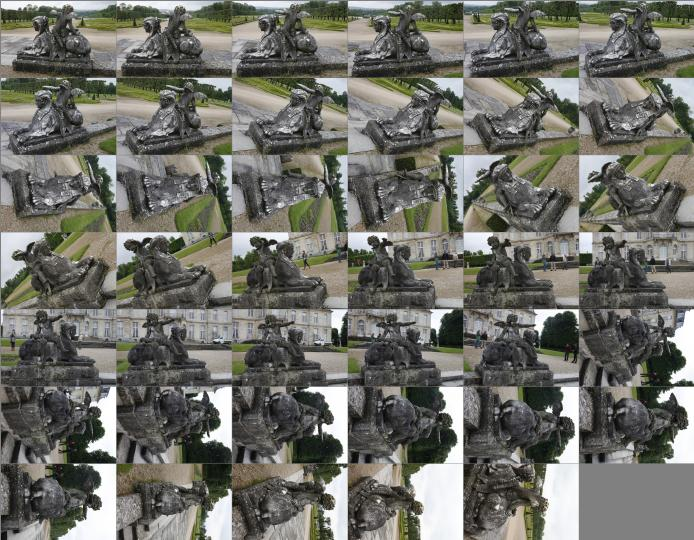
\includegraphics[width=120mm]{FIGS/Ange/Panel.jpg}
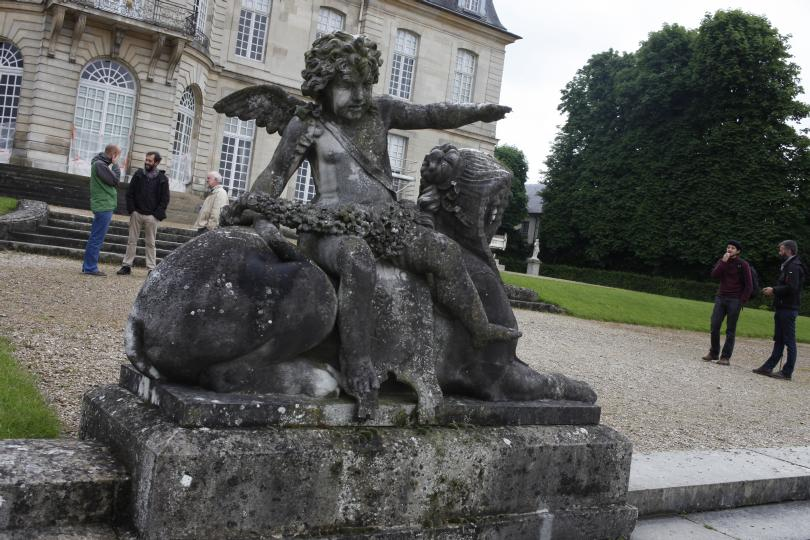
\includegraphics[width=120mm]{FIGS/Ange/SMALL_MG_1044.JPG}
\end{center}
\caption{The Angel statue used for the {\tt C3DC QuickMac} command}
\label{FIG:Angel:Flog}
\end{figure}


Here is a possible command using a dataset of $41$ images of a statue :


\begin{verbatim}
mm3d C3DC QuickMac _MG_10.*JPG Ori-All2/ Masq3=AperiCloud_All2_selectionInfo.xml
\end{verbatim}


The result are presented on figure~\ref{FIG:Angel:Result}. Computation time was $12$ min with a $8$ processor machine.




\begin{figure}[H]
\begin{center}
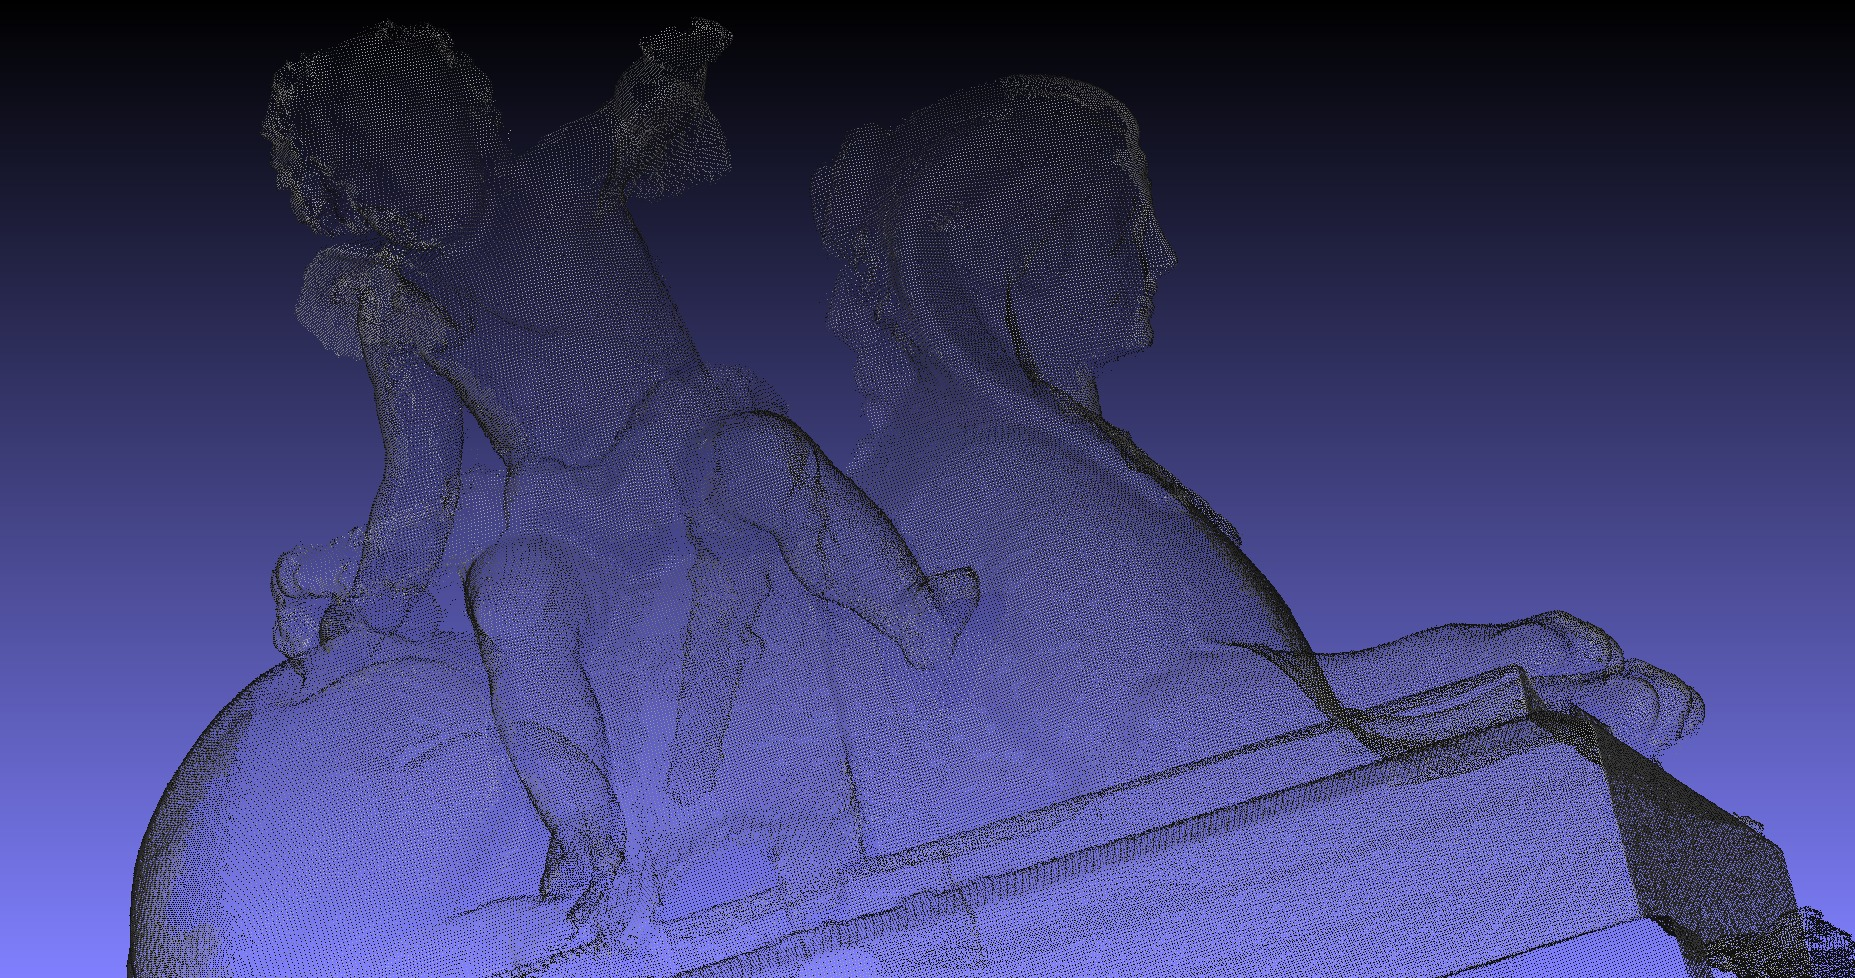
\includegraphics[width=100mm]{FIGS/Ange/snapshot00.jpg}
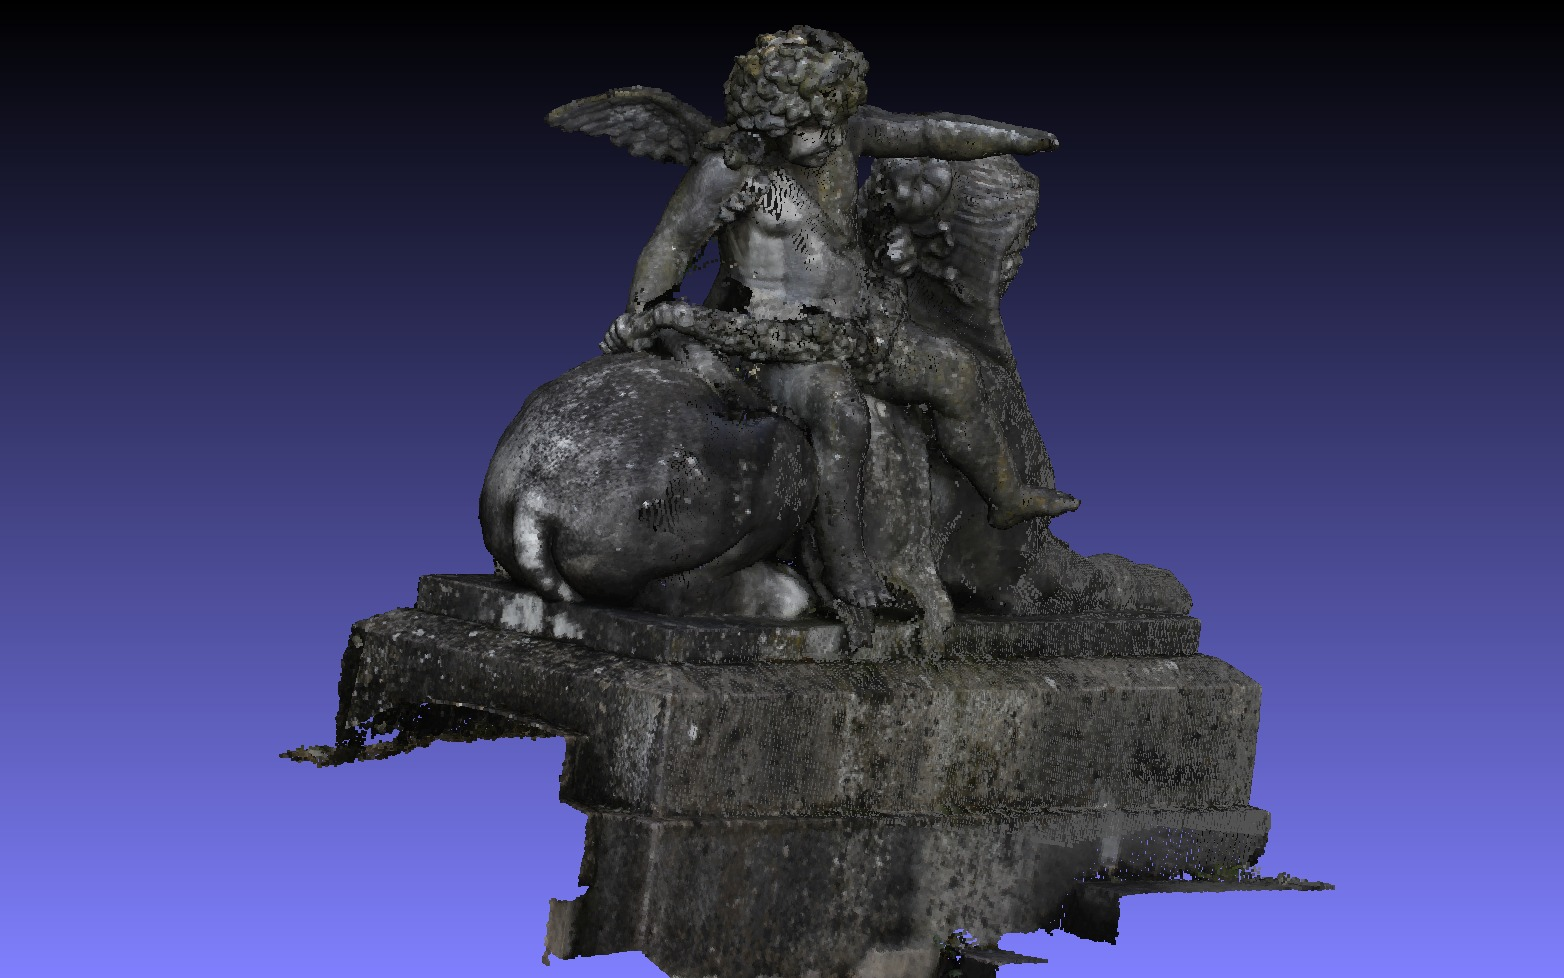
\includegraphics[width=100mm]{FIGS/Ange/snapshot01.jpg}
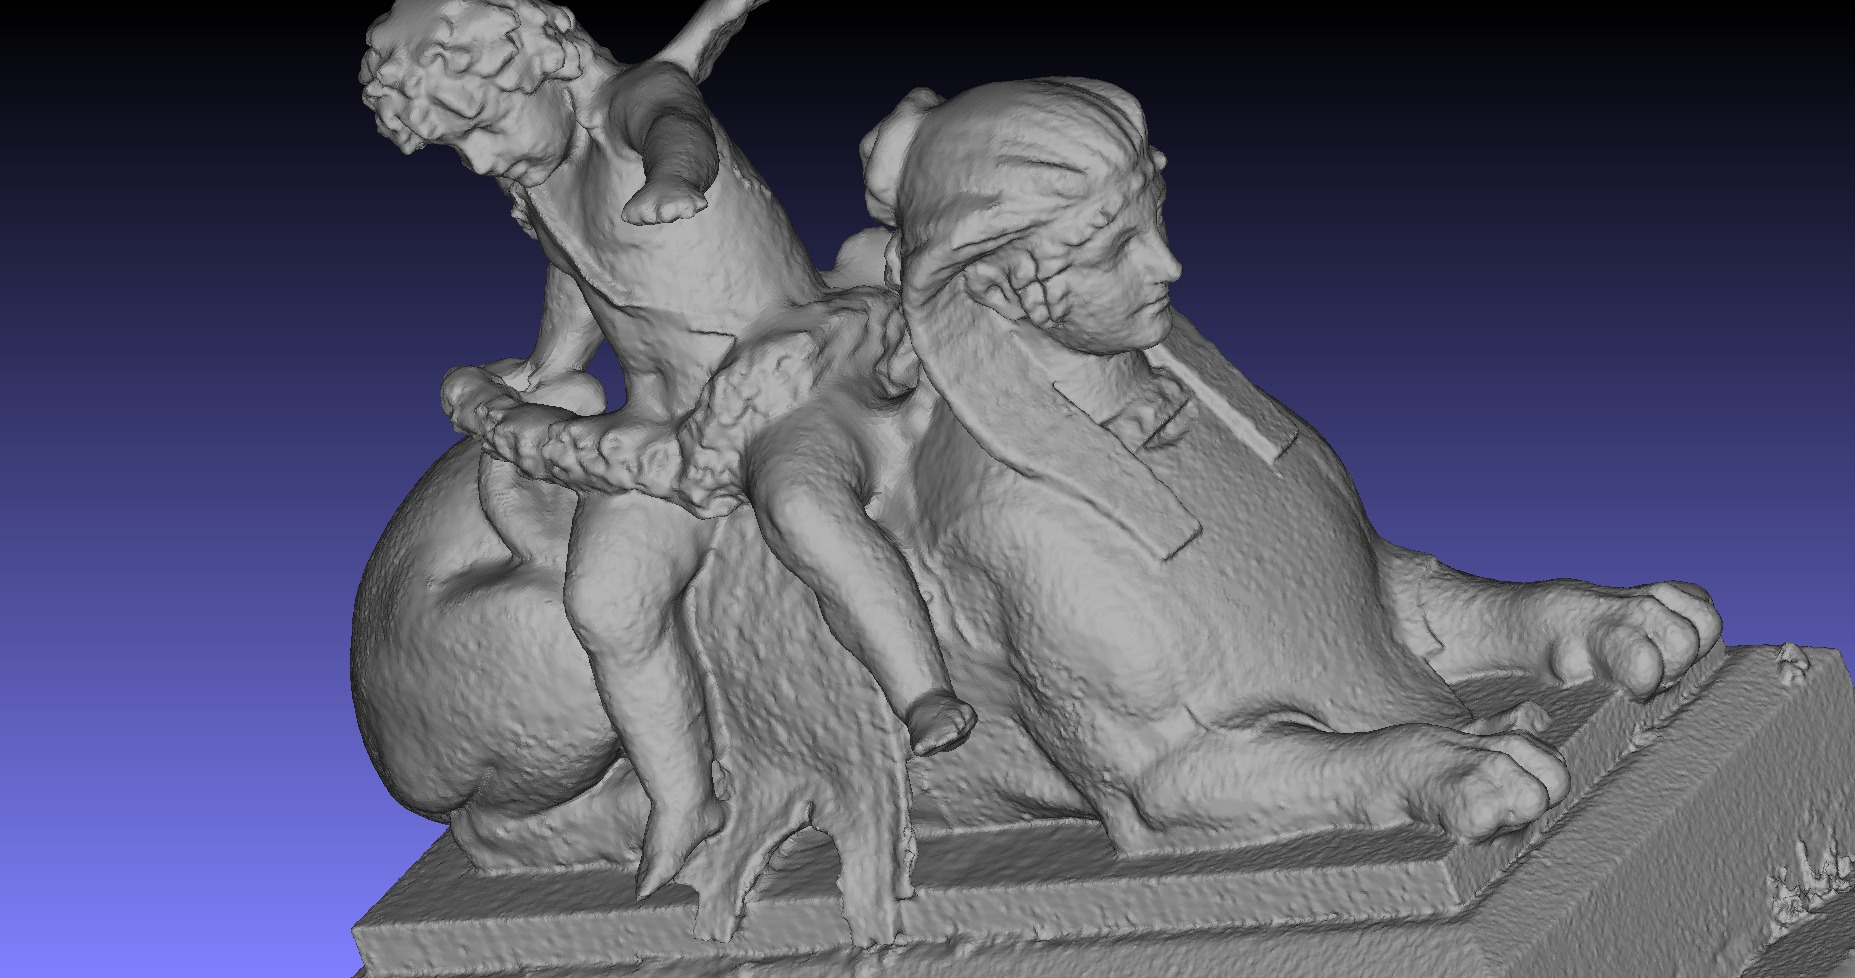
\includegraphics[width=100mm]{FIGS/Ange/snapshot201.jpg}
\end{center}
\caption{Result of {\tt C3DC QuickMac} command: point cloud, coloured point cloud, meshed poind cloud}
\label{FIG:Angel:Result}
\end{figure}

%-------------------------------------------------------------------
%-------------------------------------------------------------------

\section{Post-processing tools - mesh generation and texturing}

\subsection{Mesh generation}

Note: this tool is still under development, for now, it is recommended to use it with Filter option set to false. To use this tool, if compiling from sources, run {\tt cmake} with {\tt BUILD\_POISSON} option activated.
\begin{verbatim}
    cmake -DBUILD_POISSON=ON
\end{verbatim}

{\tt TiPunch} command creates a mesh from a point cloud. The point cloud has to be in .ply format and has to store normal direction for each point.
This commands performs two steps:
\begin{itemize}
\item mesh generation
\item mesh filtering\\*
\end{itemize}
Mesh generation is built as a call to {\tt PoissonRecon} binary from Misha Khazdan (for more information on M. Khazdan's code and research: \url{http://www.cs.jhu.edu/~misha/Code/PoissonRecon/} )
It has mainly one important parameter: the depth of reconstruction. {\tt PoissonRecon} solves the Poisson equation with a discretization of space into a voxel grid. The depth $d$ parameter defines the size of the voxel grid, as grid is $2^d$ x $2^d$ x $2^d$ voxels.
As a result, a higher depth will lead to a higher level of detail in the final mesh.\\*

As {\tt PoissonRecon} can sometimes generate wrong mesh parts, mesh filtering is necessary to deletes parts of the mesh which are too far from point cloud.
Mesh filtering makes the assumption that point cloud ply has been generated using {\tt C3DC} command. But one can also use {\tt Nuage2Ply} (with Normale option) and MergePly to generate compatible point cloud. In this case, you can desactivate mesh filtering, with option Filter=0.
To filter the mesh, depth images are used (there location is recovered from Pattern and C3DC mode). To reduce computing time, use a subset of the whole images set (typically 8 to 12 in statue configuration), by choosing the right pattern.

\begin{verbatim}
mm3d TiPunch -help
*****************************
*  Help for Elise Arg main  *
*****************************
Mandatory unnamed args :
  * string :: {Ply file}
Named args :
  * [Name=Pattern] string :: {Full Name (Dir+Pat)}
  * [Name=Out] string :: {Mesh name (def=plyName+ _mesh.ply)}
  * [Name=Bin] bool :: {Write binary ply (def=true)}
  * [Name=Depth] INT :: {Maximum reconstruction depth for {\tt PoissonRecon} (def=8)}
  * [Name=Rm] bool :: {Remove intermediary Poisson mesh (def=false)}
  * [Name=Filter] bool :: {Filter mesh with distance (def=false)}
  * [Name=Mode] string :: {C3DC mode (def=Statue)}
  * [Name=Scale] INT :: {Z-buffer downscale factor (def=2)}
  * [Name=FFB] bool :: {Filter from border (def=true)}
\end{verbatim}

Syntax is:

\begin{itemize}
  \item ply file, with normal direction computed for each point
  \item {\tt Pattern}, needed if Filter=true, set of images to filter mesh (we use depth images computed by C3DC)
  \item {\tt Out}, output mesh filename
  \item {\tt Bin}, output mesh ply format (ascii or binary, true means binary)
  \item {\tt Depth}, Maximum reconstruction depth for PoissonRecon
  \item {\tt Rm}, remove output of {\tt PoissonRecon} (mainly if Filter=true)
  \item {\tt Filter}, do we filter mesh
  \item {\tt Mode}, needed if Filter=true, mode of C3DC (needed for PIMs- directory)
  \item {\tt Scale}, Z-buffer downscale factor, used for filtering (a bigger downscale factor speeds up process, but is less accurate)
  \item {\tt FFB}, Filter from border: force filtering to start from mesh borders (it avoids creating holes)
\end{itemize}

\subsection{Texturing the mesh}

{\tt Tequila} computes a UV texture image from a ply file, a set of images and their orientations. Ply file has to be a mesh, and can be the result of {\tt TiPunch} (but not the direct result of {\tt C3DC}).
Here again, using the whole set of images is not necessary. Choosing a subset of the whole images is recommended (8 to 12 images can give good results, in statue mode).\\*

{\tt Tequila} performs following steps:

\begin{itemize}
    \item load data
    \item compute zbuffers
    \item choose which image is best for each triangle
    \item filter mesh according to visibility (optional)
    \item graph-cut optimization (optional)
    \item write UV texture
    \item write ply file with uv texture coordinates\\*
\end{itemize}

Choosing which image is best for each triangle can be done with three different criterions:
\begin{itemize}
\item   best angle between triangle normal and image viewing direction (parameter Crit=Angle, by default, and recommended)
\item   best stretching of triangle projection in image (parameter Crit=Stretch)
\item   best acute angle of triangle projection in image (parameter Crit=AAngle)\\*
\end{itemize}

For the angle criterion, expressed in degrees, a threshold is set to avoid using images that view a triangle with a low incidence (parameter Angle).
It means that if the angle between triangle normal and image viewing direction is higher than $Angle$, the image will not be used for texturing.\\*

{\tt Tequila} has also two modes, which refer to texture computing strategies: $basic$ and $pack$. In the $basic$ mode, all images from the set are stored in the uv texture, and if necessary are downscaled. Each image is masked with the zbuffer, to store a minimum of significant information.
In the $pack$ mode, each image is divided in small regions, and only useful regions are packed into the uv texture, in an optimal way. This mode leads to smaller images, and gives better texture quality.

\begin{verbatim}
mm3d Tequila -help
*****************************
*  Help for Elise Arg main  *
*****************************
Mandatory unnamed args :
  * string :: {Full Name (Dir+Pat)}
  * string :: {Orientation path}
  * string :: {Ply file}
Named args :
 * [Name=Out] string :: {Textured mesh name (def=plyName+ _textured.ply)}
 * [Name=Bin] bool :: {Write binary ply (def=true)}
 * [Name=Optim] bool :: {Graph-cut optimization (def=false)}
 * [Name=Lambda] REAL :: {Lambda (def=0.1)}
 * [Name=Iter] INT :: {Optimization iteration number (def=2)}
 * [Name=Filter] bool :: {Remove border faces (def=false)}
 * [Name=Texture] string :: {Texture name (def=plyName + _UVtexture.jpg)}
 * [Name=Sz] INT :: {Texture max size (def=4096)}
 * [Name=Scale] INT :: {Z-buffer downscale factor (def=2)}
 * [Name=QUAL] INT :: {jpeg compression quality (def=70)}
 * [Name=Angle] REAL :: {Threshold angle, in degree, between triangle normal and image viewing direction (def=90)}
 * [Name=Mode] string :: {Mode (def = Pack)}
 * [Name=Crit] string :: {Texture choosing criterion (def = Angle)}
\end{verbatim}

Relevant parameters are:
\begin{itemize}
\item {\tt Angle}, threshold for maximum angle between normal and viewing direction
\item {\tt Mode}, choose between Basic and Pack (see upper)
\item {\tt Crit}, choose between Angle, Stretch, and AAngle (see upper)
\item {\tt Scale}, which allow to speed up computation (higher downscale factor leads to faster computation).
\item {\tt Sz}, which will force texture size, to conform with graphic card capacity (see GL\_MAX\_TEXTURE\_SIZE if available)
\item {\tt QUAL}, the jpeg compression quality, which allows to compact UV texture image.
\item {\tt Optim}, post-processing step, to gather neighbouring triangles with the same image texture (graph-cut algorithm, detailed below)
\item {\tt Lambda}, weighting factor for graph-cut optimization
\item {\tt Iter}, number of iteration steps for optimization\\*
\end{itemize}

In most cases, illumination variations, BRDF variations upon directions, and surface shape will lead a simple texturing algorithm to produce artefacts in texture: two adjacent triangles can be assigned two different texture images, while only one texture image for both triangles might be better.
In some rare cases (no illumination variation, etc.), these artefacts won't be visible. Also if a texture equalization is applied (process that will be included one day in the {\tt MicMac} tools) these artefacts won't happen, or should be less visible.\\*

To limit jumps between several texture images in adjacent triangles, an optimization can be performed as a post-processing step. This optimization is stated as a multi-label energies graph-cut.
Each triangle is assigned a likelihood term (here, angle to image viewing direction or projected triangle stretching).
Two adjacent triangles define a graph edge, and a coherence term is assigned to this edge (here, the difference between mean texture in each triangle).
$\lambda$ parameter (Lambda) is the weight between likelihood term and coherence term.\\*

\begin{figure}[H]
\begin{center}
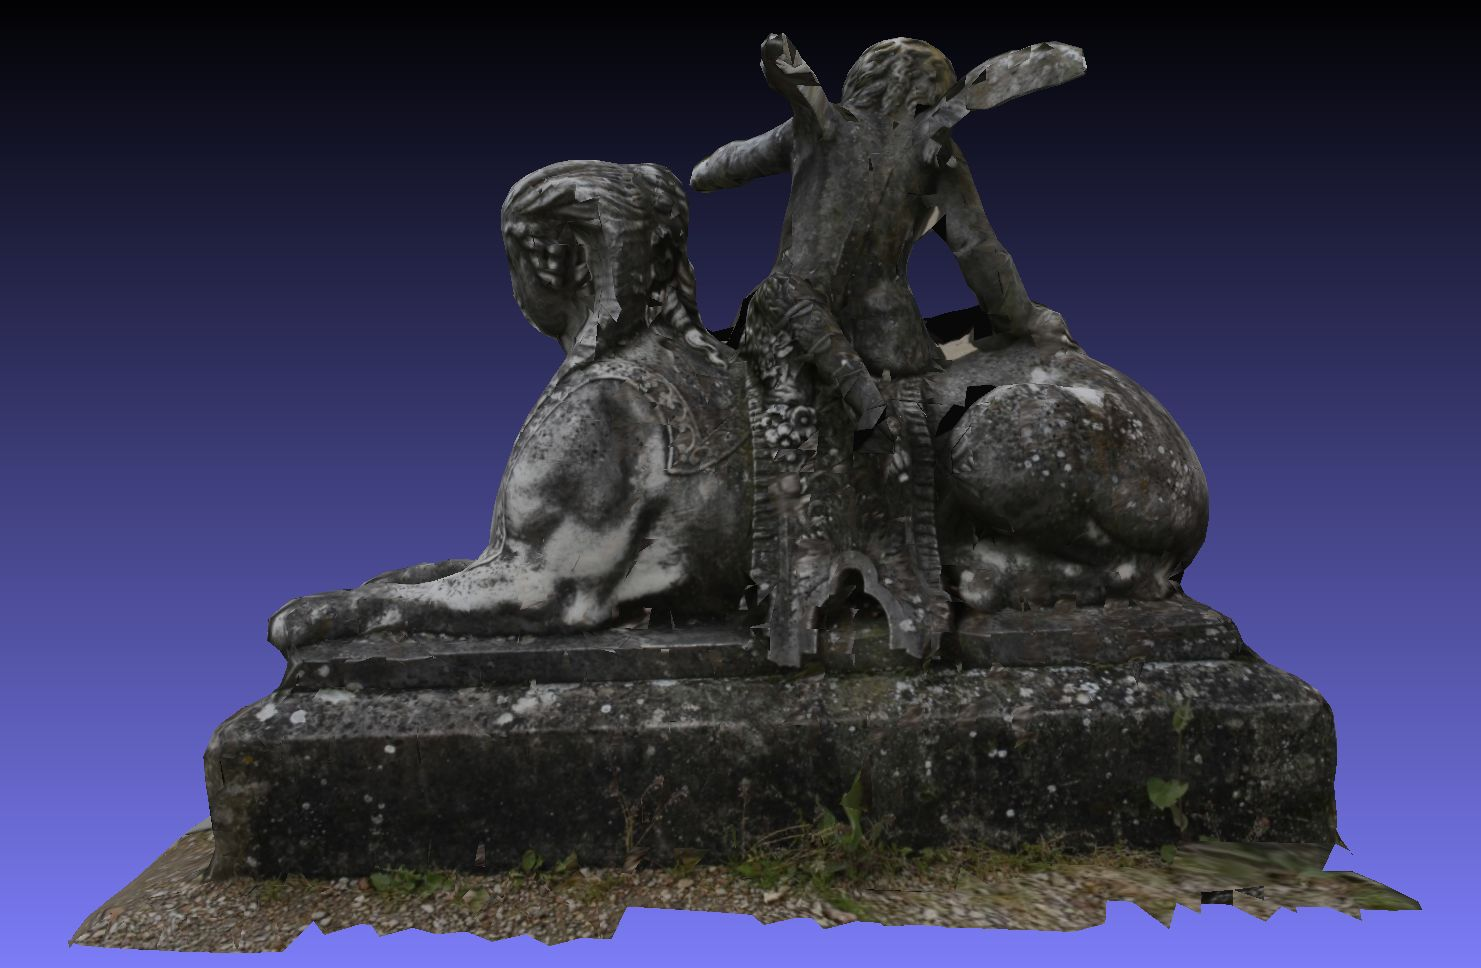
\includegraphics[width=110mm]{FIGS/Ange/Tequila.jpg}
\end{center}
\caption{The Angel statue mesh textured with {\tt Tequila} command}
\label{FIG:Angel:Tequila}
\end{figure}
%-------------------------------------------------------------------
%-------------------------------------------------------------------

\section{Parallelizing Apero}

For now works only with linear orientation.

\subsection{Parallelizing Apero}

The new tool {\tt Liquor} (for LInear QUick ORientation) accelerate the computation of orientation. The acceleration comes
from two aspects:

\begin{itemize}
   \item  it uses a hierarchical building of orientation, which make the computation in $N Log N$ instead of $N^2$
   \item  at the low level of the pyramid, it parallelizes the computation of subset on the several processors.
\end{itemize}

The syntax :

\begin{verbatim}
mm3d Liquor -help
*****************************
*  Help for Elise Arg main  *
*****************************
Mandatory unnamed args :
  * string :: {Full name (Dir+Pat)}
  * string :: {Calibration Dir}
Named args :
  * [Name=SzInit] INT :: {Sz of initial interval (Def=50)}
  * [Name=OverLap] REAL :: {Prop overlap (Def=0.1) }
\end{verbatim}

An example of use with the data set of figure~\ref{FIG:Liquor:DataMap} :

\begin{verbatim}
mm3d Liquor CAM2_0.* Ori-Calib/
\end{verbatim}


With these $150$ images the computation time is $20 min$ instead of $1h10min$ with traditional {\tt Tapas}.

\begin{figure}[H]
\begin{center}
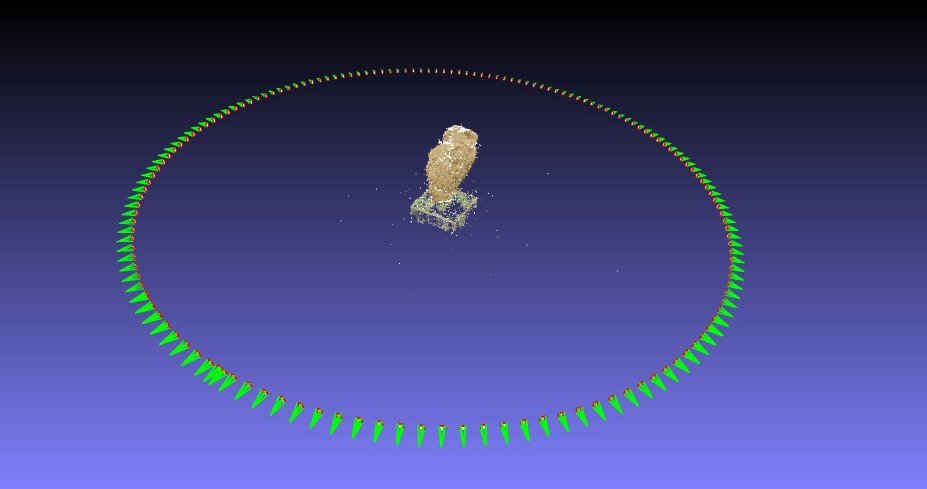
\includegraphics[width=100mm]{FIGS/Ange/LineAcq.jpg}
\end{center}
\caption{Linear acquisition used for {\tt Liquor} command}
\label{FIG:Liquor:DataMap}
\end{figure}


